	\newpage
\section{Projektowanie}		%3
%Napisać z jakich narzędzi będziemy korzystać (kompilator, język programowania), git, biblioteki dodatkowe, itp.
%Opisać szczegółowe ustawienia kompilatora (jeśli są), powiązania z bibliotekami, itp.
%Narysować graf, UML, diagram klas, schemat działania algorytmu
%Jeśli zadanie zakłada przedstawienie jakiegoś narzędzia (np. git, AI) należy opisać sposób jego używania

\subsection{Implementacja Merge Sort}


Do zaimplementowania Merge Sorta zostanie użyty Język \texttt{C++} z kompilatorem \texttt{g++}. Wersja standardu \texttt{C++} to \texttt{C++20}. Jako, że projekt ma być rozdzielony na dwa pliki, zostanie zastosowany \texttt{CMake} w celu automatyzacji procesu budowania. \texttt{CMake} pozwala na generowanie plików budujących dany projekt, zgodnie z określoną konfiguracją. Oszczędza to programiście, szczególnie przy większych projektach, manualne pisanie Makefileów.
Plik konfiguracyjny \texttt{CMakeLists.txt} może wyglądać jak na rysunku

\begin{lstlisting}[caption=Plik konfiguracyjny CMake, label={lst:cmakelists}, language=C++]
	cmake_minimum_required(VERSION 3.15)
	
	set(PROJECT_NAME proj1)
	
	project(${PROJECT_NAME} VERSION 0.1 LANGUAGES CXX)
	
	set(CMAKE_CXX_STANDARD 20)
	set(CMAKE_CXX_STANDARD_REQUIRED ON)
	set(CMAKE_EXPORT_COMPILE_COMMANDS True)
	set(CMAKE_RUNTIME_OUTPUT_DIRECTORY ${CMAKE_CURRENT_LIST_DIR}/out)
	
	add_subdirectory(src)
	
\end{lstlisting}

Edytorem będzie program Neovim. Jest to terminalowy edytor tekstu z możliwością poszerzenia funkcjonalności przy użyciu wszelkiego rodzaju pluginów. Wybrany został, dlatego że jest on już skonfigurowany na moim komputerze zgodnie z moimi preferencjami.

\subsection{Git}

Dla ułatwienia pracy, zastosowany został front-end dla gita o nazwie lazygit. Jest to terminalowy program, którego główną zaletą jest łatwa nawigacja przy użyciu klawiatury. Ponadto, jest on lekki i szybki.

\subsection{Doxygen}

Konfiguracja dla Doxygena jest wygenerowana przy użyciu programu doxywizard, pokazany na rys. \ref{fig:doxywizard}, pozwalającego na graficzne zmienianie ustawień. Po wygenerowaniu konfiguracji, Doxygen wywoływany jest przy użyciu komendy.

\begin{figure}[H]
	\centering
	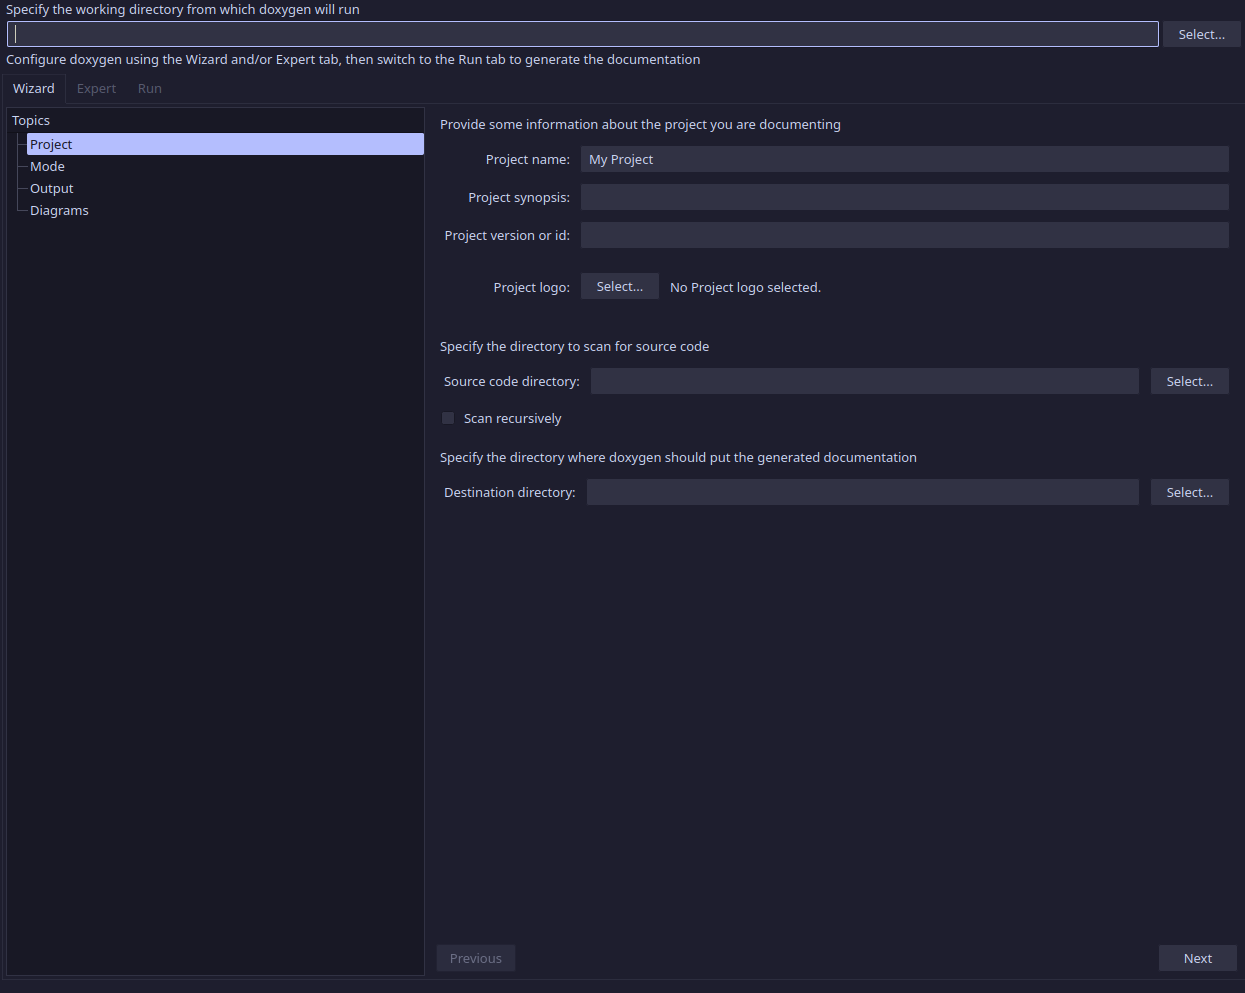
\includegraphics[width=1\textwidth]{images/doxywizard.png}
	\caption{\centering{Interfejs programu doxywizard}}
	\label{fig:doxywizard}
\end{figure}

\subsection{Google Test}

Google Test został dodany do projektu jako biblioteka w \texttt{CMake}, co zostało ukazane na listingu nr.~\ref{lst:gtestcmake}. Framework jest automatycznie pobierany i instalowany przy konfiguracji.

\begin{lstlisting}[caption=Dodanie Google Test do projektu, label={lst:gtestcmake}, language=C++]
include(FetchContent)
	FetchContent_Declare(
			googletest
			URL https://github.com/google/googletest/archive03597a01ee50ed33e9dfd640b249b4be3799d395.zip
	)
FetchContent_MakeAvailable(googletest)

\end{lstlisting}

Pliki źródłowe testów znajdują się we własnym folderze, więc też trzeba do niego dodać \texttt{CMakeLists}, jak widać na listingu nr.~\ref{lst:testscmake}

\begin{lstlisting}[caption=Dodanie Google Test do projektu, label={lst:testscmake}, language=C++]
file(GLOB_RECURSE SRC_FILES *.cpp *.h)
set(TESTS_EXECUTABLE ${PROJECT_NAME}_tests)

enable_testing()

add_executable(${TESTS_EXECUTABLE} ${SRC_FILES})

target_link_libraries(
	${TESTS_EXECUTABLE} PUBLIC
	${PROJECT_NAME}_lib
	GTest::gtest_main
)

\end{lstlisting}

Plik wykonywalny testów jest linkowany do - oprócz samego frameworka - biblioteki jaka jest wygenerowana z klasy \texttt{MergeSorter}, o której więcej w sekcji nr.~\ref{sec:MergeSorter}.
